\documentclass[12pt]{article}
\usepackage{amsmath}
\usepackage{amssymb}
\usepackage{graphicx}
\usepackage{color}
\usepackage{setspace}

\begin{document}
\pagestyle{plain}
\doublespacing

\title{Aircraft Queueing Problem}
\author{John DeSalvo}
\maketitle

\tableofcontents

\section{Abstract}
In this paper, we explore the 1989 Aircraft Queueing Problem from the Mathematical Contest in Modeling. The objective is to minimize the cost for both the airline and the passengers in terms of time. The approach is a meta-heuristic inspired by neural networks. The determination of whether a given aircraft takes off on time or is added to a queue is based on the linear separability principles of the perceptron algorithm. Data for specific days, months, and years are generated via Monte Carlo simulation. Some algorithms involving modular arithmetic are used to assign data to specific dates accurately. A greedy algorithm that favors the airline is first examined to model how time delays accumulate. A specific dataset is used for "training" so that further randomly generated data can fit the model. 

\section{Non-Technical Summary}
The hypothetical airline for this problem has seven different types of aircrafts with capacities of 100, 150, 200, 250, 300, 350, and 400 seats. Every 15 minutes, a flight is scheduled which may have more or less passengers than the capacity of the plane. We first see what happens if the airline does not allow a plane to leave until it is completely full. We then see how time delay accumulates as time progresses. We use this information to determine a maximum that the total costs for the passengers and the airline can be as a means to decide whether or not each aircraft will take off as scheduled or be added to a queue.

\section{Introduction}
During a day at an airport, a flight is scheduled every fifteen minutes with a variable number of passengers scheduled for each flight. The aircrafts have capacities of 100, 150, 200, 250, 300, 350, and 400 seats so an aircraft with a capacity close to the number of passengers scheduled for each flight is assigned to that flight. In this situation, there is access to a hypothetical database that contains the following information:
\begin{enumerate}
    \item the time the aircraft is scheduled for takeoff
    \item the actual time of takeoff
    \item the number of passengers on board
    \item the capacity of the aircraft
    \item the number of passengers who depart at the next stop
    \item the number of passengers who are schduled to board at the next stop
    \item the scheduled time of arrival at the next stop
\end{enumerate}
The problem description is to simply "develop and analyze a mathematical model that take into account both the travelers' and the airlines' satisfaction." More precisely, what this means is that the objective is to minimize the cost for the passengers in terms of time spent waiting and to minimze the cost for the airline in terms of the number of seats unfilled. For each time-step $t_{i}$ of $15$ minutes there is: \\
$c$ := the aircraft capacity that varies from $100$ to $400$ in increments of $50$ \\
$n$ := the number of people scheduled for a flight \\
$m$ := the number of people scheduled to make a connection at the next flight (depart or board) \\
$t_{s}$ := the scheduled pushback time \\
$t_{a}$ := the actual pushback time \\
$t_{f}$ := the average duration of a flight
\\
For the satisfaction of the passengers, the expression for the cost is: \\
$(t_{a} - t_{s})(n + m)$ \\
\\
For the satisfaction of the airline, the expression for the cost is: \\
$t_{f}[(c - n) + (c - n + m)]$ \\
\\
For both parties involved the goal is to minimize the cost. With respect to the passengers, we take this to be the additional time spent waiting multiplied by the number of people waiting for the corresponding amount of time. With respect to the airline, this is the number of seats unfilled multiplied by the time each seat spends in the air unfilled. The reasoning here is so that both expressions are in the same units and thus are comparable. \\

\section{Methods}
\subsection{Generating a Databse}
Within a week of either Christmas or Thanksgiving, the number of passegners increases proportionally to how close it is to the holiday. This is according to a variant of the sinc function modified ad-hoc to increase the density closer to holidays. \\
$f(t) = |sinc(4t)| + \frac{\pi}{2}$ \\
 
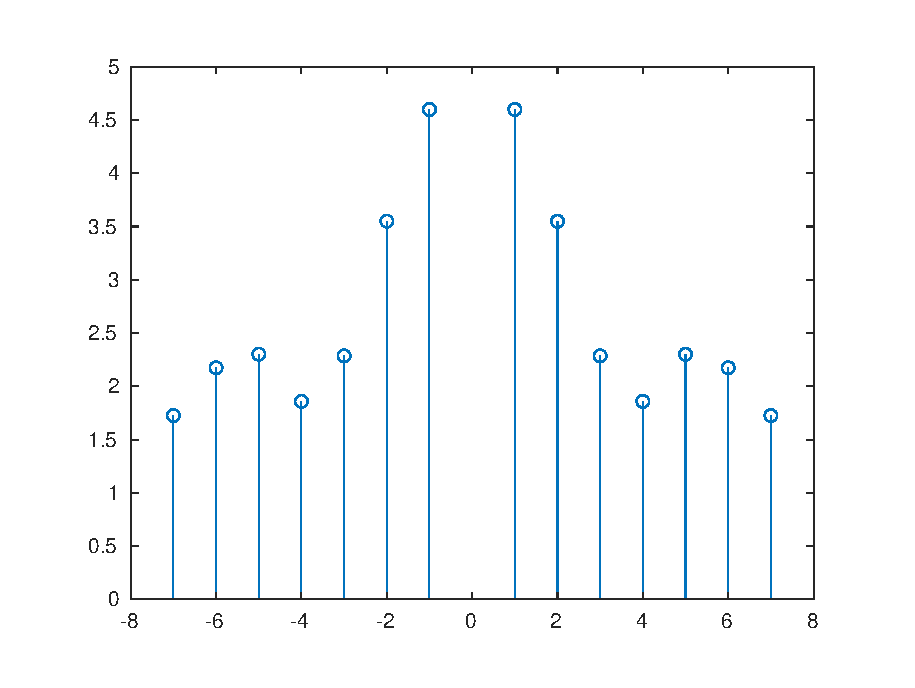
\includegraphics{sinc.eps}

In addition to generating database fields for a given day, a function is implemented to generate data for every day for a given year. Modular arithmetic is used to determine the appropriate number of days in a month for that year. It is also used to determine when Thanksgiving is for the given year. The spike in the number of passengers can be observed when running the Monte Carlo simulation to generate a database for a whole year. \\
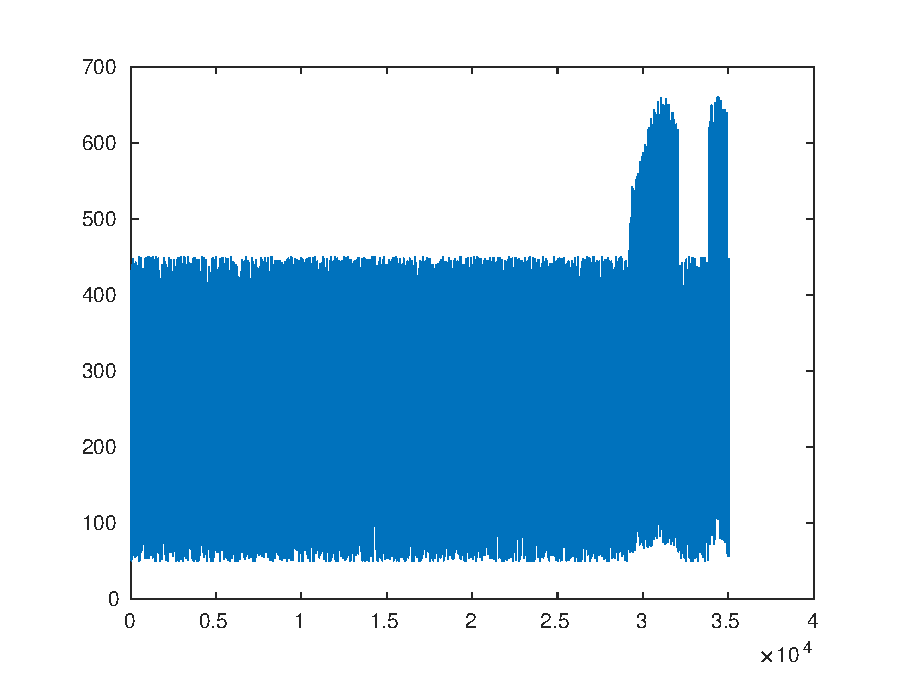
\includegraphics{yeardist.eps}

\sloppy
\definecolor{lightgray}{gray}{0.5}
\setlength{\parindent}{0pt}
\begin{verbatim}
function AC = ACDByear(year)
AC = [];
	for i = 1:12
        switch i
            case 1
                J = 31;
            case 2
                if mod(year, 4) == 0
                    J = 29;
                else
                    J = 28;
                end
            otherwise
               if sqrt(i) == round(sqrt(i)) || mod(i, 5) == 1
                   J = 30;
               else
                   J = 31;
               end
        end
        for j = 1:J
            ac = ACDBday(i, j, year);
            AC = vertcat(AC, ac);
        end
    end
end
\end{verbatim}

\begin{par}
This generates the database of information for all scheduled aircrafts on a given day. The number of customers in a day is random from a range, clustered around the max of that range close to Thanksgiving and Christmas. The objective is to minimize the amount of time each passenger spends waiting and maximize the amount of passengers in an AC. Suppose a flight is scheduled every 15 minutes.
\end{par} \vspace{1em}
\begin{verbatim}
function AC = ACDBday(month, day, year)
    actype = 100:50:400;
    % number of discrete time intervals, each is 15 minutes
    N = 96;
    % function determining the density of increase in passengers aroung the
    % holidays
    f = @(x) abs(4*sin(4*x)./x) + pi/2;
    % determine the date of thanksgivng that year
    incr =  abs(year-2019);
    for i = 1:incr
        if mod(year, 4) == 0
            incr = incr + 2;
        else
            incr = incr + 1;
        end
    end
    % week of Thanksgiving
    if month == 11
        hday = 7 - mod(7, incr) + 21;
    % week of Christmas
    elseif month == 12 && abs(25-day) < 6
        hday = 25;
    else
        hday = 0;
    end

    for i = 1:N
        cap = randi([1 7]);
        n = randi([actype(cap)-50 actype(cap)+50]);
        for j = 1:5
            switch j
                % aircraft type
                case 1
                    AC(i, j) = actype(cap);
                % number of passengers
                case 2
                    if hday
                        AC(i, j) = round(f(abs(day-hday)+1)*n/(exp(1)/2));
                    else
                        AC(i, j) = n;
                    end
                % number of passengers leaving at the next stop
                case 3
                    AC(i,j) = randi([0 AC(i, j-1)]);
                % number of passengers boarding at the next stop
                case 4
                    AC(i, j) = randi([0 AC(i, j-2) - AC(i, j-1)]);
                % timesetp, t
                otherwise
                    AC(i, j) = i;
            end
        end
    end
end
\end{verbatim}

\subsection{Model for Training}
Since database information is generating using random integers, a dataset for a single day is used to model the behavior of the general system. This dataset was selected after several Monte Carlo simulations. The data is then processed via an algorithm that favors the airline and the costs for both the airline and the passengers are measured. If the number of people scheduled for a flight is greater than the capacity of the aircraft, an excess number of people are forced to wait for another aircraft with vacant seats (for simplicity, this model assumes all flight from the airport arrive at the same destination as the next stop). If there are vacant seats on a scheduled flight, an aircraft will wait until all seats are filled. If possible, the seats will be filled by excess passengers from previous flights. When there are still vacant seats and no passengers waiting to fill them, an aircraft is then added to the queue. An aircraft at the beginning of the queue will be dequeued when a scheduled flight has enough excess passengers to fill its vacant seats. \\
\\
This approach leads to error with resepct to the passengers that compounds: \\
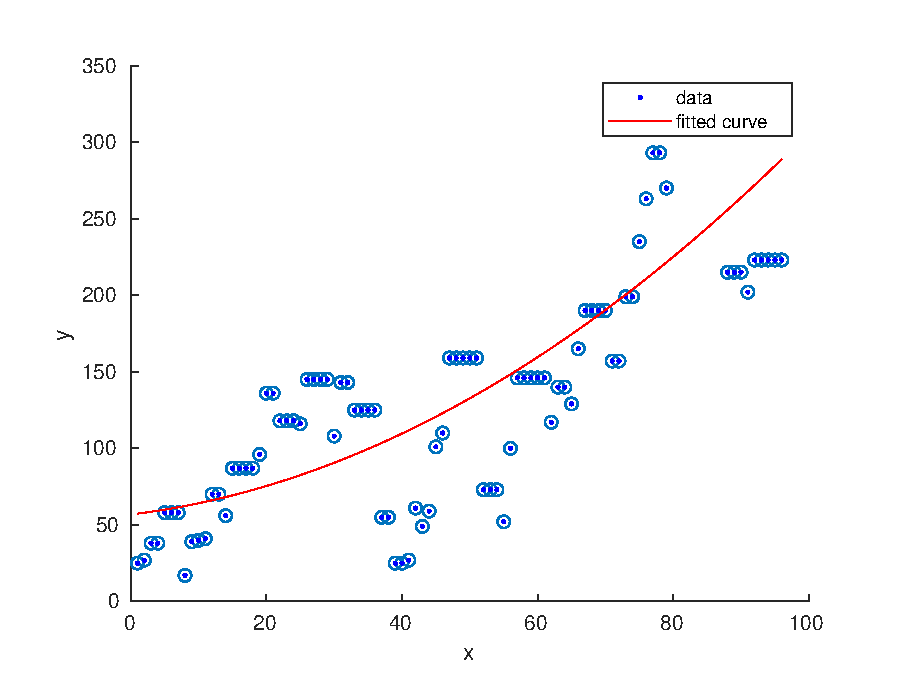
\includegraphics{poly2.eps}
\\
However, the cost of unfilled seats remains a random distribution because there is no accumulation. The waiting time for the passengers is then compared to the hypothetical loss of revenue for the airlines had it not filled vacant seats. \\
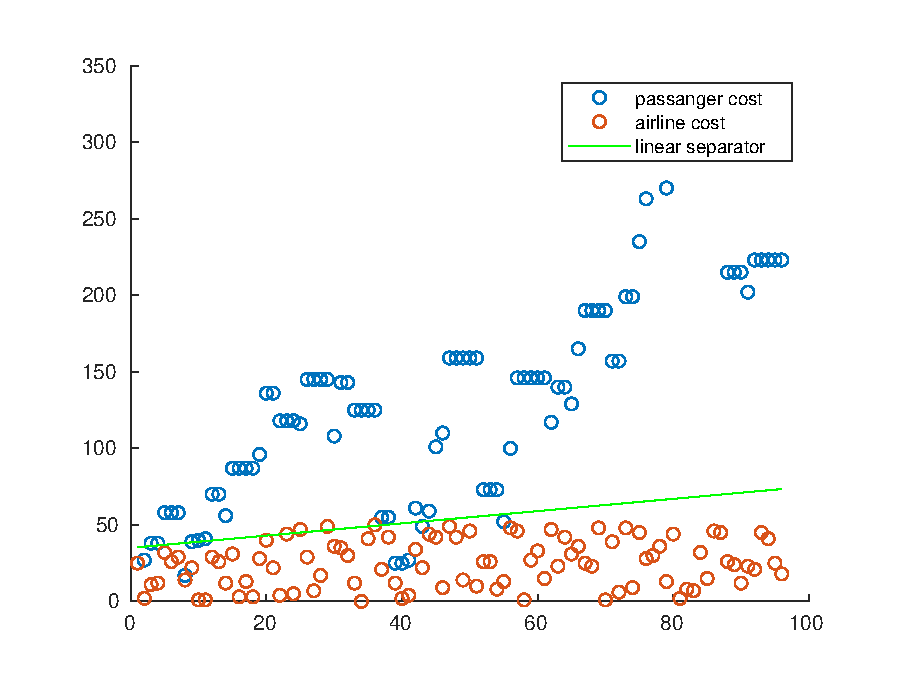
\includegraphics{linsep.eps}
\\
Following the perceptron approach, linear separation is determined to differentiate cost for the passengers from cost for the airline. The function for this line is determined heuristically and by inspection rather than allowing a neural network to converge. The equation for the line is determined to be: \\
$0.4t + 35$ \\
This function is then used to train subsequent datasets to ensure that the total error does not exceed this boundary.

\section{Results}
The simulation is then run for a single day where the total error does not exceed the boundary according to the training model.

\begin{verbatim}
AC = ACDBday(4, 21, 2019);
nErr = AC(:,1) - AC(:,2);
f = @(t) 0.4*t  + 35;
t = 1:length(AC);
q = 0;
ncum = 0;
tcum = 0;

for i = t
    if heaviside(nErr(i))
        ncum = ncum + nErr(i);
        tcum = ncum;
    else
        q = q + 1;
        tcum = abs(nErr(i));
    end
    if tcum + ncum > f(t(i))
        q = q-1;
        if q < 0
            q = 0;
        end
        tcum = 0;
        ncum = 0;
        pf(i) = 1;

    else
        pf(i) = 0;
    end
    Q(i) = q;
    N(i) = ncum;
    T(i) = tcum;
    NT(i) = tcum + ncum;
end
plot(t, f(t), t, NT)
\end{verbatim}

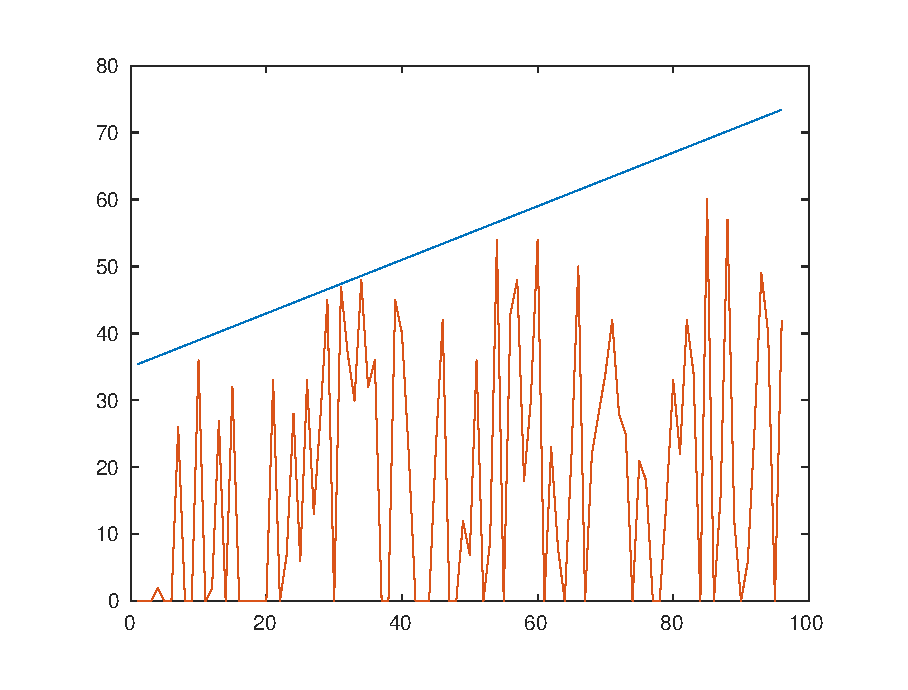
\includegraphics{linPF_01.eps}

Running the simulation for a whole year, the queue accumulates as the airline tries to fill seats but the error is bounded by the linear function.

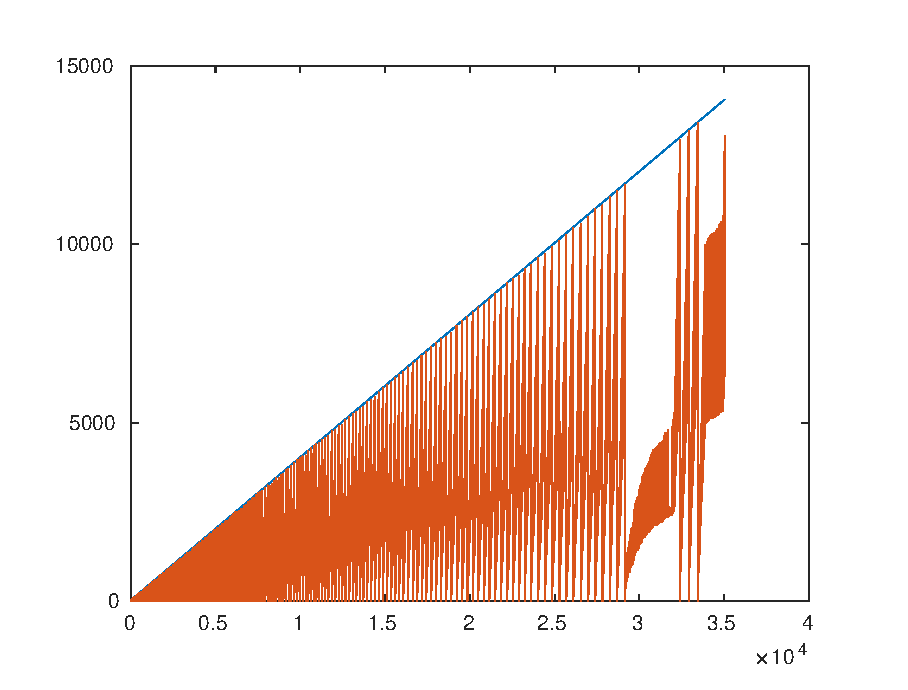
\includegraphics{linPF_02.eps}

In the following figure, the pass/fail condition of the aircraft is shown as values of "0" or "1". In other words, it is shown whether each aircraft is algorithmically determined to take off or be added to the queue. Larger queue size at the end of the year, around the holidays accomodates the larger number of passengers.

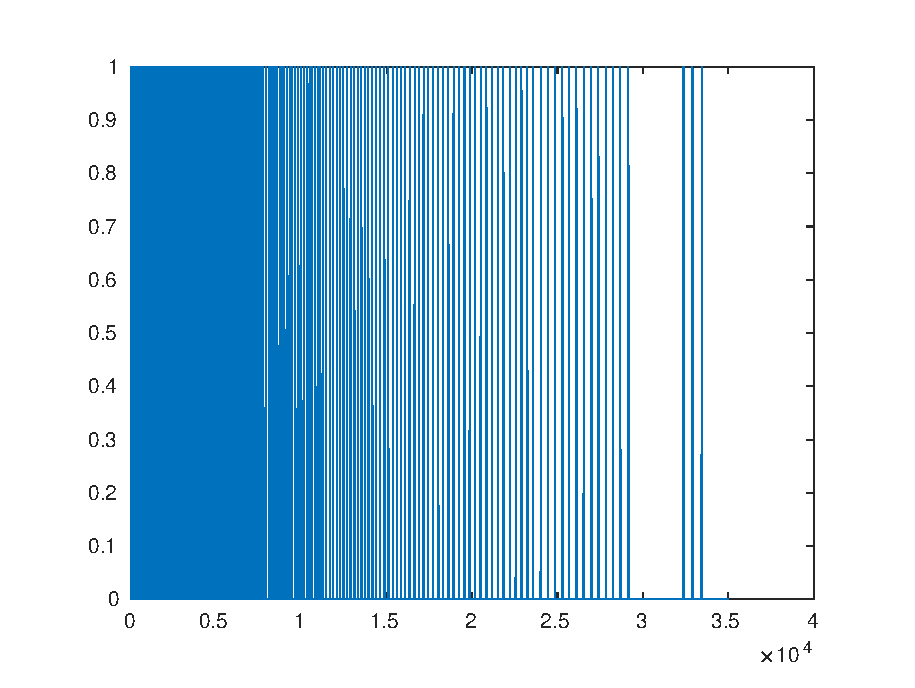
\includegraphics{pf.eps}

\end{document}
